% Created 2022-04-14 Thu 10:49
% Intended LaTeX compiler: xelatex
\documentclass[11pt]{article}
\usepackage{graphicx}
\usepackage{longtable}
\usepackage{wrapfig}
\usepackage{rotating}
\usepackage[normalem]{ulem}
\usepackage{amsmath}
\usepackage{amssymb}
\usepackage{capt-of}
\usepackage{hyperref}
\usepackage{color}
\usepackage{listings}
\usepackage[newfloat]{minted}
\usepackage[utf8]{inputenc}
\usepackage[table,xcdraw]{xcolor}
\usepackage{paralist}
\usepackage{datetime2}
\usepackage{graphicx}
\usepackage{lscape}
\usepackage{longtable}
\usepackage{hyperref}
\usepackage[a4paper, left=3cm, right=3cm, top=2cm]{geometry}
\usepackage{fancyhdr}
\usepackage{listings}
\usepackage{textcomp}
\usepackage{enumitem}
\usepackage{algorithm}
\usepackage{algpseudocode}
\setlist{noitemsep}
\setlength{\columnseprule}{0.2pt}
\definecolor{mygreen}{rgb}{0,0.6,0}
\definecolor{mygray}{rgb}{0.5,0.5,0.5}
\definecolor{mymauve}{rgb}{0.58,0,0.82}
\lstset{ backgroundcolor=\color{white}, basicstyle=\footnotesize, breaklines=true, captionpos=b, commentstyle=\color{mygreen}, escapeinside={\%*}{*)},keywordstyle=\color{blue}, stringstyle=\color{mymauve},}
\author{Olivier Lischer}
\date{\today}
\title{Design Patterns - Summary}
\hypersetup{
 pdfauthor={Olivier Lischer},
 pdftitle={Design Patterns - Summary},
 pdfkeywords={},
 pdfsubject={},
 pdfcreator={Emacs 28.1 (Org mode 9.5.1)}, 
 pdflang={English}}
\begin{document}

\pagestyle{fancy}
\fancyhf{}
\fancyhead[R]{SEP2-FS}
\fancyhead[L]{Design Patterns - Summary}
\fancyfoot[CE,CO]{\leftmark}
\fancyfoot[R]{\thepage}
\fancyfoot[L]{Olivier Lischer}

\begin{titlepage}
  \begin{center}
    {\Huge Design Patterns - Summary} \\
    \vspace{8 cm}

    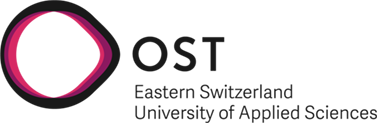
\includegraphics[height=4cm]{./img/ost-logo.png}

    \vspace{4 cm}
    Semester: Spring 2022
    \vspace{1 cm}

    Version: 0.1.0 \\
    Date: \DTMnow \\
    \vspace{3 cm}
    School of Computer Science\\
    OST Eastern Switzerland University of Applied Sciences
  \end{center}
\end{titlepage}
\newpage
\tableofcontents
\newpage


\section{Introduction}
\label{sec:org67a3615}
\subsection{Most important quotes}
\label{sec:org22f1716}
In the introduction the basics of object-oriented programming are explained.
Therefore, for many this is easy to read.
However, some important statements are made.

\begin{quote}
Favor object composition over class inheritance
\end{quote}

Because it is very difficult to make the correct abstraction often the base class(es) are not complete or have too much in it.
With object composition you don't have this problem.

\begin{quote}
Program to an interface, not an implementation
\end{quote}
If you implement against interfaces you can test your class with unit tests.
If you implement against a fixed implementation you can not change this behavior at anytime.


\subsection{The design patterns}
\label{sec:orga82a798}

Class Design Patterns deal with the relationships between classes and their subclasses.
The Object Design Patterns with the object relationships which can be changed at runtime.

\begin{figure}[htbp]
\centering
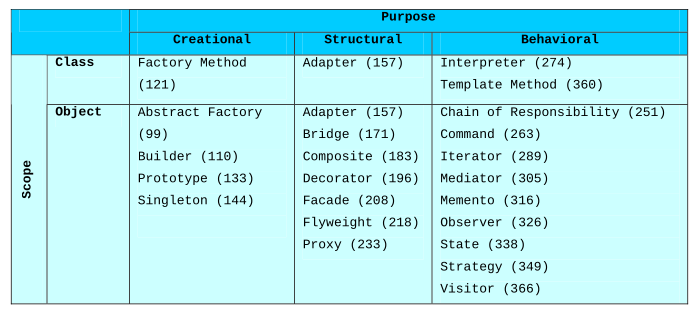
\includegraphics[width=.9\linewidth]{img/design_pattern_space.png}
\caption{\label{fig:design-pattern-space}Design pattern space}
\end{figure}

\subsection{The Most common causes of redesign}
\label{sec:org9fb5aee}

A list of the most common causes of redesign and how you could solve the problem.

\begin{enumerate}
\item Creating an object by specifying a class explicitly.

Try to avoid creating objects explicitly otherwise you are bound to this decision.

\href{../../../../roam/20220413195148-design_pattern_abstract_factory.org}{Design Pattern - Abstract Factory}, \href{../../../../roam/20220413195351-design_pattern_factory_method.org}{Design Pattern - Factory Method}, \href{../../../../roam/20220413195501-design_pattern_prototype.org}{Design Pattern - Prototype}

\item Dependence on specific operations

Try to avoid to hard code how you want to satisfy a request.
Example: Do not hard code how a specific button should perform.

\href{../../../../roam/20220413200329-design_pattern_chain_of_responsibility.org}{Design Pattern - Chain of Responsibility}, \href{../../../../roam/20220413200356-design_pattern_command.org}{Design Pattern - Command}
\item Dependence on hardware and software platform

Try to avoid implementing against a specific HW or API.

Example: Linux \& Windows does not have the same Windows System.
Provide an abstraction in which the underlying system is not relevant.

\href{../../../../roam/20220413195148-design_pattern_abstract_factory.org}{Design Pattern - Abstract Factory}, \href{../../../../roam/20220413200620-design_pattern_bridge.org}{Design Pattern - Bridge}

\item Dependence on object representations or implementations

You should never bother how the inside of class works while using it.
Otherwise, you might need to change things when the class is changing its inner live.

\href{../../../../roam/20220413201034-design_pattern_builder.org}{Design Pattern - Builder}, \href{../../../../roam/20220413201100-design_pattern_iterator.org}{Design Pattern - Iterator}, \href{../../../../roam/20220413201128-design_pattern_strategy.org}{Design Pattern - Strategy}, \href{../../../../roam/20220413201147-design_pattern_template_method.org}{Design Pattern - Template Method}, \href{../../../../roam/20220413201212-design_pattern_visitor.org}{Design Pattern - Visitor}

\item Algorithmic dependencies

Do not hard code the algorithm.
Try to encapsulate the algorithm in a class.
Then you can replace it every time you want.

\href{../../../../roam/20220413201034-design_pattern_builder.org}{Design Pattern - Builder}, \href{../../../../roam/20220413201100-design_pattern_iterator.org}{Design Pattern - Iterator}, \href{../../../../roam/20220413201128-design_pattern_strategy.org}{Design Pattern - Strategy}, \href{../../../../roam/20220413201147-design_pattern_template_method.org}{Design Pattern - Template Method}, \href{../../../../roam/20220413201212-design_pattern_visitor.org}{Design Pattern - Visitor}

\item Tight coupling

Try to avoid tight coupling.
Otherwise, it is hard to reuse the class.

\href{../../../../roam/20220413195148-design_pattern_abstract_factory.org}{Design Pattern - Abstract Factory}, \href{../../../../roam/20220413200620-design_pattern_bridge.org}{Design Pattern - Bridge}, \href{../../../../roam/20220413200329-design_pattern_chain_of_responsibility.org}{Design Pattern - Chain of Responsibility}, \href{../../../../roam/20220413200356-design_pattern_command.org}{Design Pattern - Command}, \href{../../../../roam/20220413201512-design_pattern_facade.org}{Design Pattern - Facade}, \href{../../../../roam/20220413201546-design_pattern_mediator.org}{Design Pattern - Mediator}, \href{../../../../roam/20211103140808-observer_pattern.org}{Design Pattern - Observer}

\item Extending functionality by subclassing

This is very difficult to made it right.
Instead, use object composition to extend functionality.

\href{../../../../roam/20220413200620-design_pattern_bridge.org}{Design Pattern - Bridge}, \href{../../../../roam/20220413200329-design_pattern_chain_of_responsibility.org}{Design Pattern - Chain of Responsibility}, \href{../../../../roam/20220413202016-design_pattern_composite.org}{Design Pattern - Composite}, \href{../../../../roam/20220413202051-design_pattern_decorator.org}{Design Pattern - Decorator}, \href{../../../../roam/20211103140808-observer_pattern.org}{Design Pattern - Observer}, \href{../../../../roam/20220413201128-design_pattern_strategy.org}{Design Pattern - Strategy}

\item Inability to alter classes conveniently

Sometimes you can not modify a class (for example closed source library).
The following Design Patterns can help to work around this problem.

\href{../../../../roam/20220413202255-design_pattern_adapter.org}{Design Pattern - Adapter}, \href{../../../../roam/20220413202051-design_pattern_decorator.org}{Design Pattern - Decorator}, \href{../../../../roam/20220413201212-design_pattern_visitor.org}{Design Pattern - Visitor}
\end{enumerate}
\end{document}